	\begin{figure}[h]
		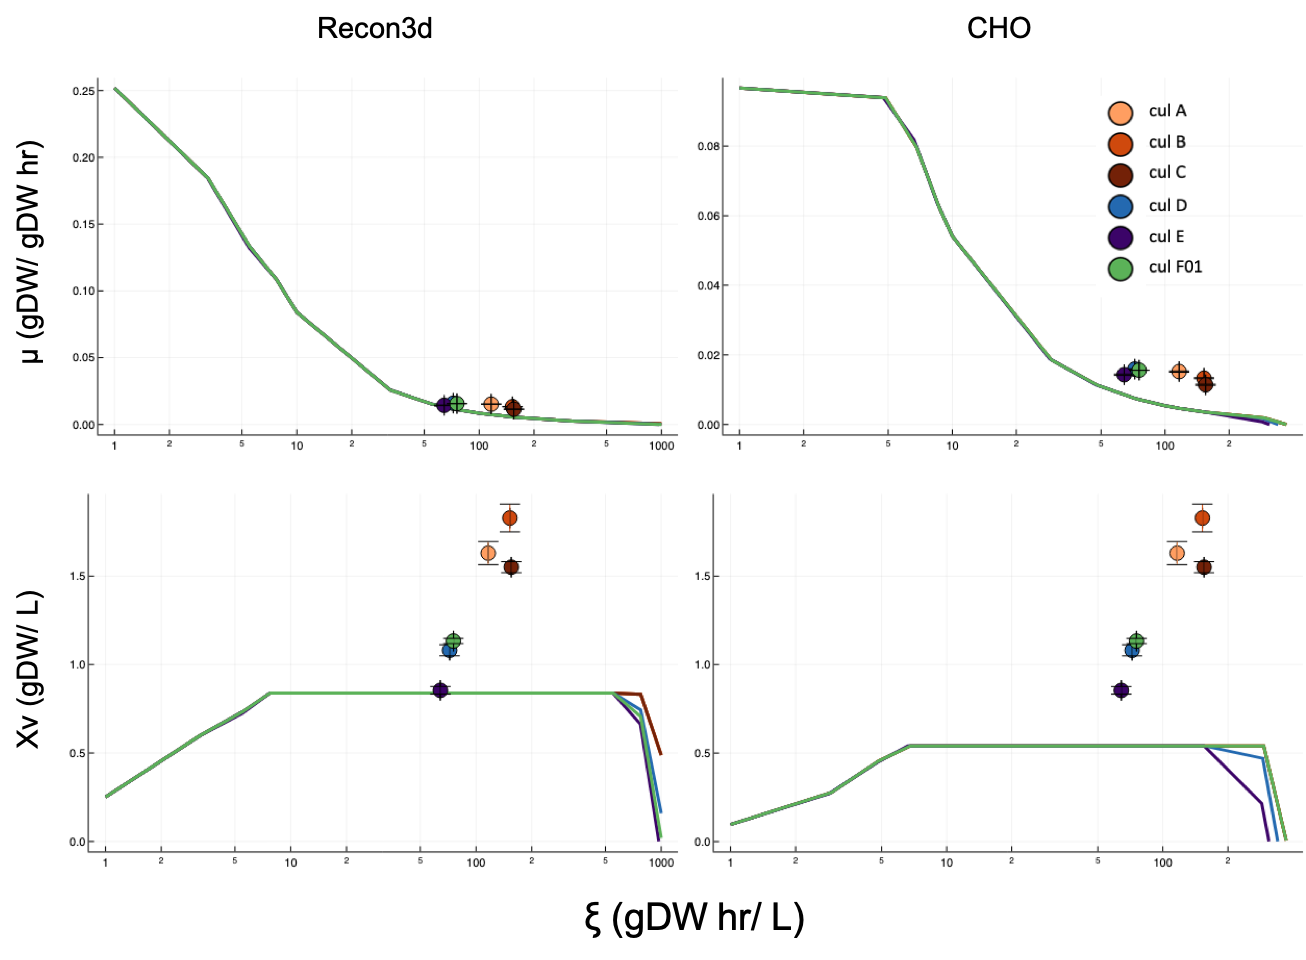
\includegraphics[scale = 0.5]{low_medium_1}
		\caption{FBAwMC results showing the growth rate, $\mu$, and the viable cell density, $Xv$, dependence of $\xi$ for the six steady states. The solid lines represent the model predictions and the colored points show the experimental results. The model data was obtained for feed mediums with low (Recon3D) and zero (CHO) concentration of phosphatidylethanolamine}
		
	\end{figure}
	
	\begin{figure}[h]
		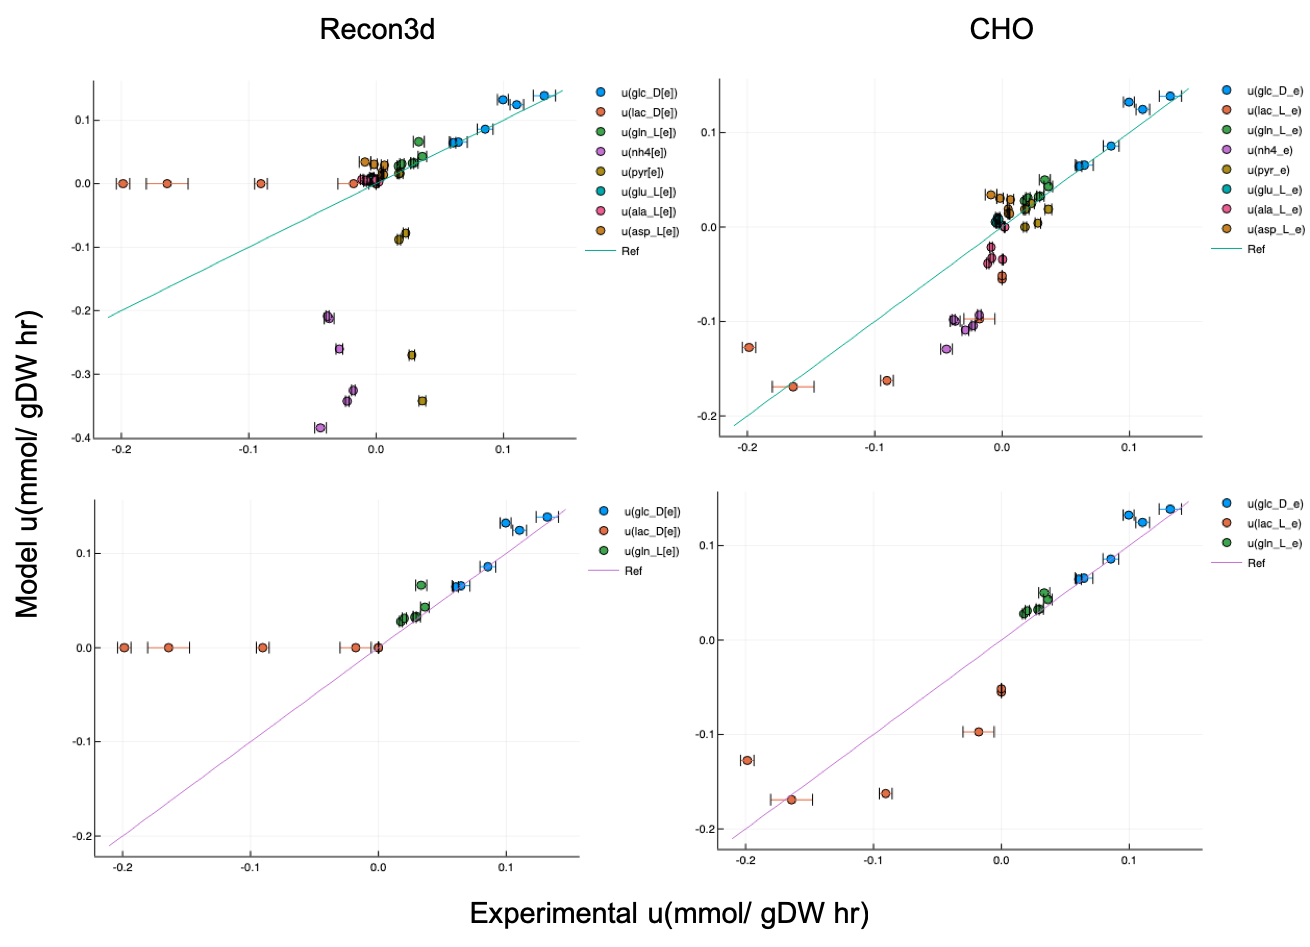
\includegraphics[scale = 0.5]{low_medium_2}
		\caption{Correlations of all the experimental uptakes, upper graphs, and a selected subset, inferior graphs, respect to the predicted value from FBAwMC with low (Recon3D) and zero (CHO) concentration of phosphatidylethanolamine.}
		
	\end{figure}
	
	\begin{figure}[h]
		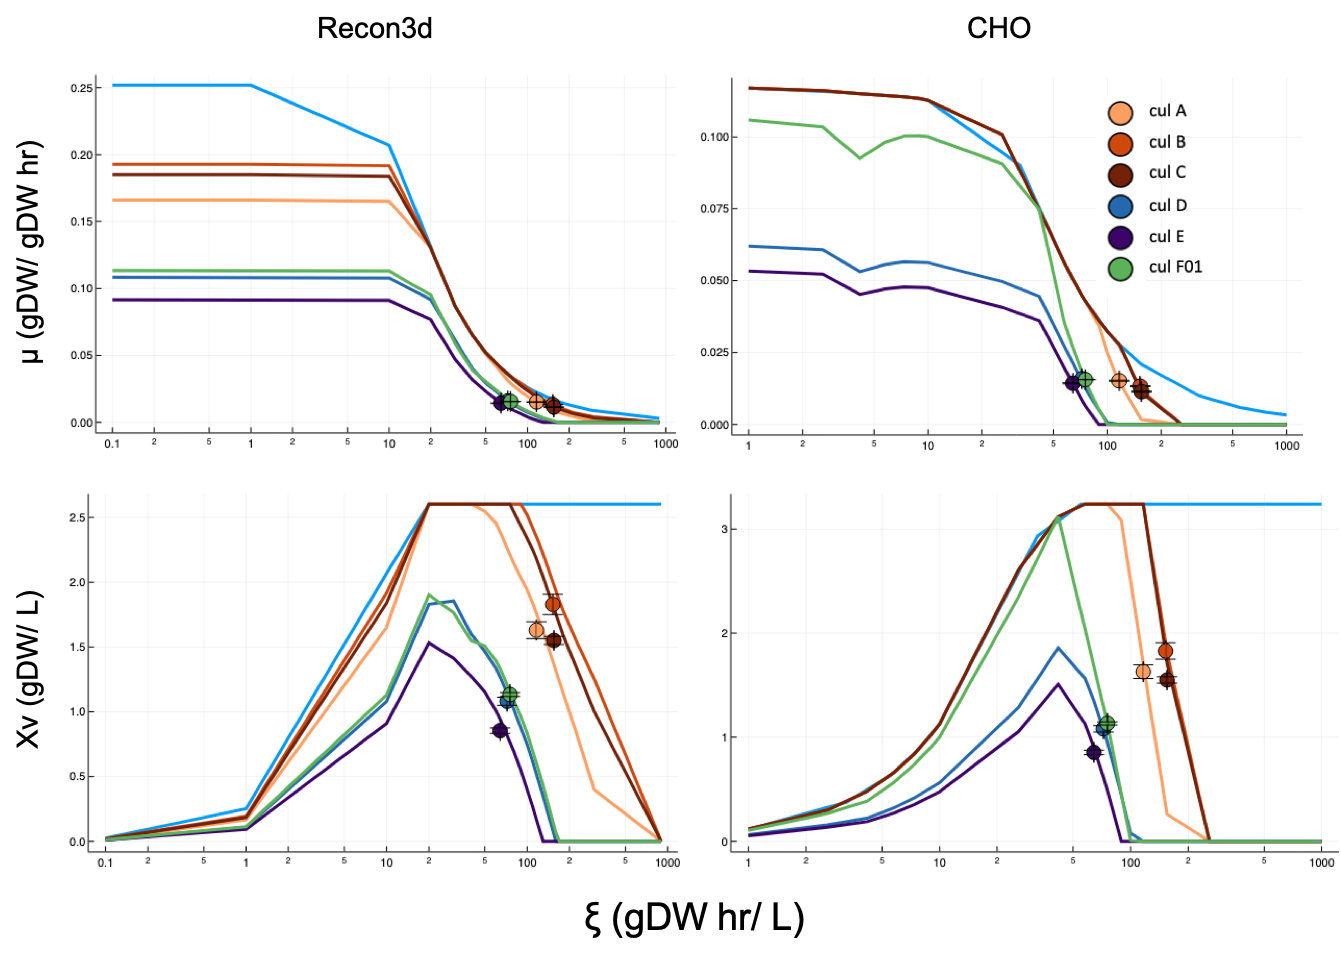
\includegraphics[scale = 0.5]{rich_medium_1}
		\caption{EP and FBA results showing the growth rate and the viable cell density dependence of $\xi$ for the six culture conditions. The solid lines represent the model predictions and the color points show the experimental results. FBA results are shown as the solid light blue line. $EP$ $\beta$ parameters was chosen, for each culture, so that the experimental $\mu$ coincides with the predicted $\mu$}
		
	\end{figure}
	
	\begin{figure}[h]
		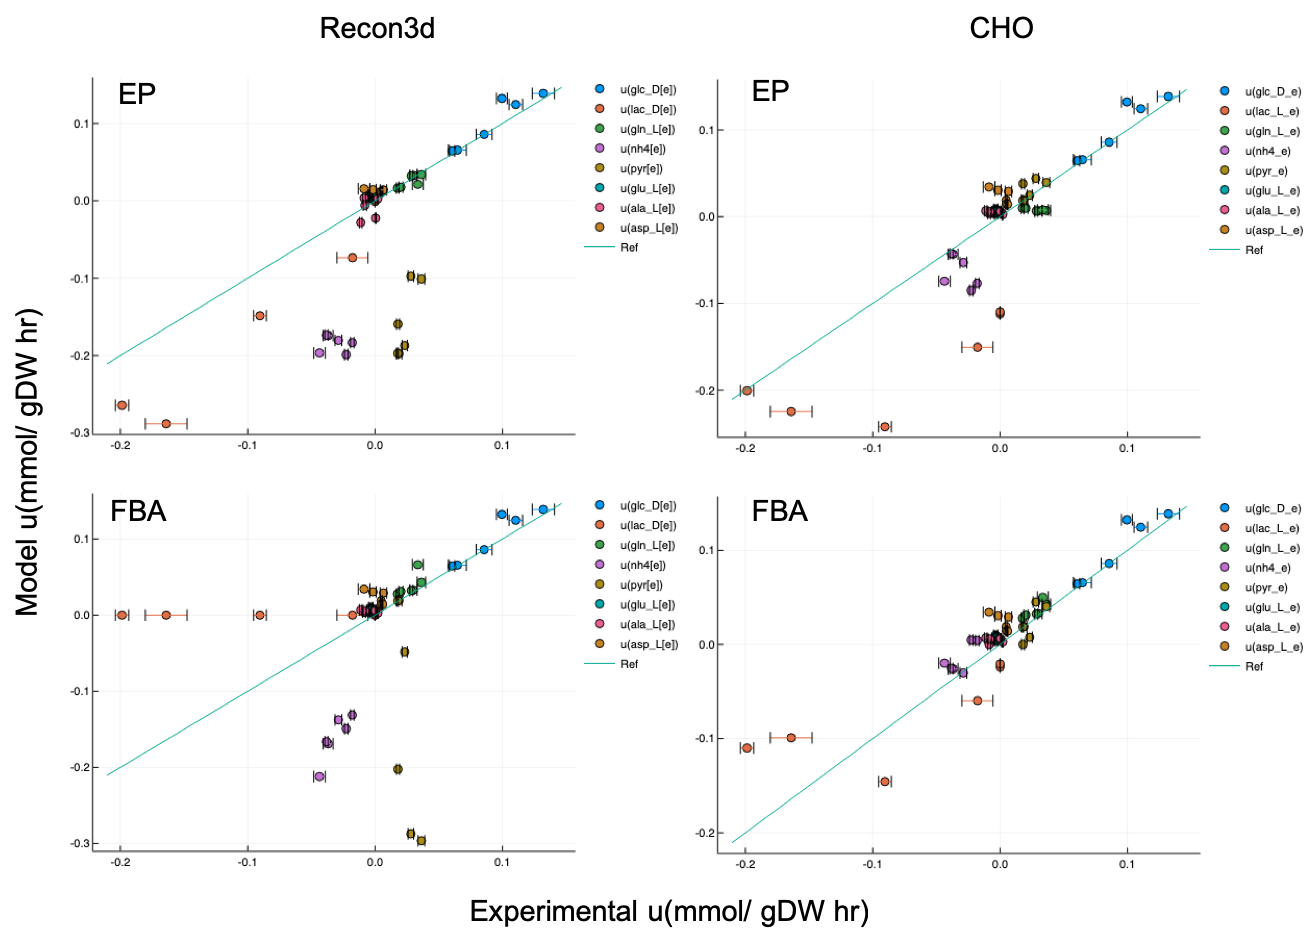
\includegraphics[scale = 0.5]{rich_medium_2}
		\caption{Correlations of all the experimental uptakes compared with the predicted value from EP and FBA for GEMs with high concentration of phosphatidylethanolamine.}
		
	\end{figure}
	
	\begin{figure}[h]
		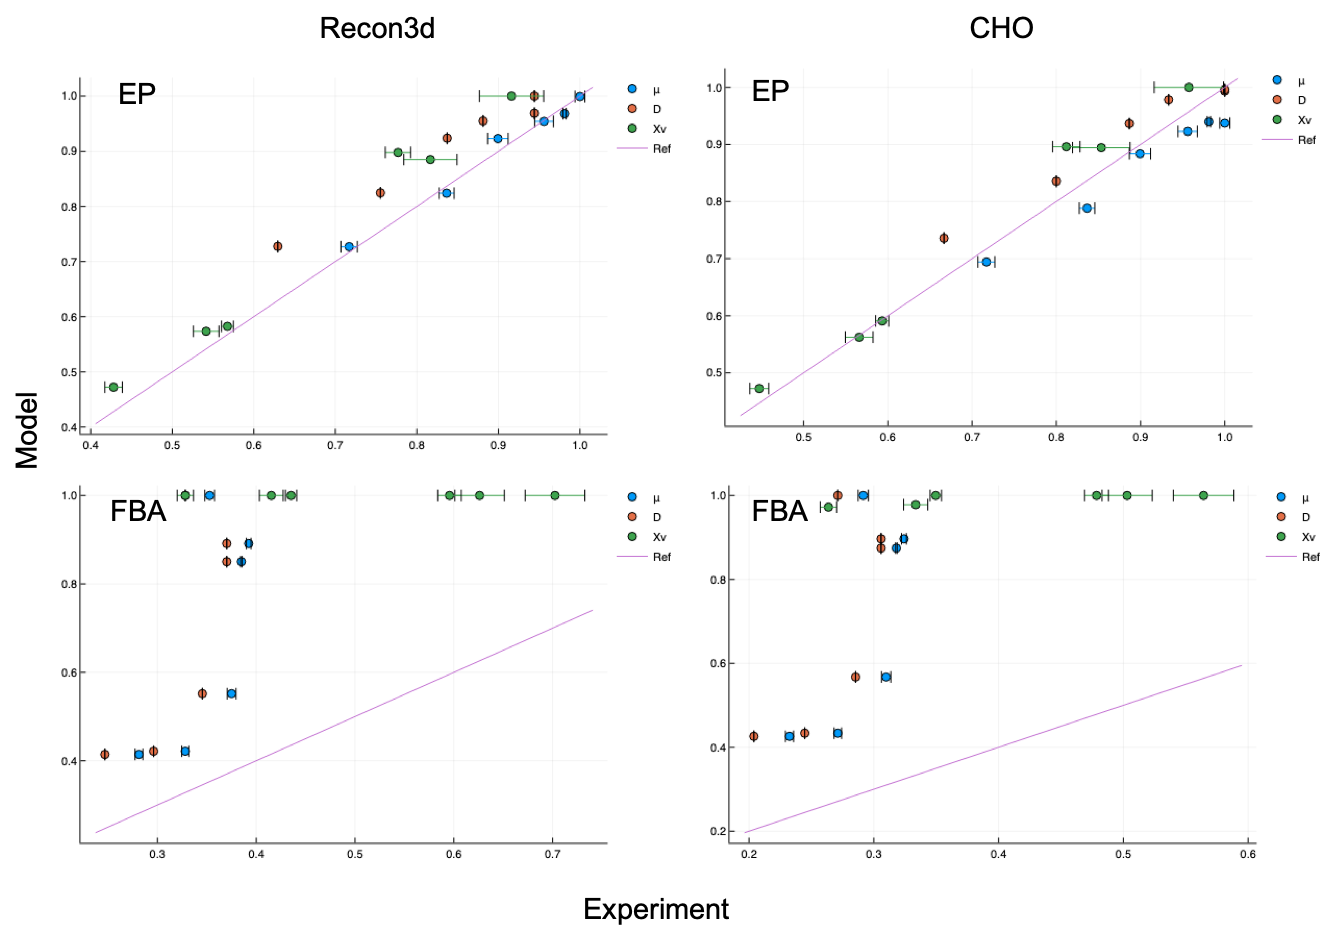
\includegraphics[scale = 0.5]{rich_medium_3}
		\caption{Normalized correlations of the experimental $\mu$, $D$ and $Xv$ compared with the predicted value from EP and FBA for GEMs with high concentration of phosphatidylethanolamine.}
		
	\end{figure}